\documentclass[a4paper,12pt]{article}
\usepackage{amsmath}
\usepackage{amsfonts}
\usepackage{amsthm}
\usepackage{amsfonts}
\usepackage{amssymb}
\usepackage{setspace}
\usepackage{graphicx}
\doublespacing
\title{Real Numbers}
\date{}
\begin{document}
\maketitle
\section{Real Numbers}
The real numbers consist of all the numbers on the real number line.
\[\mathbb R=(-\infty,\infty)\]
\subsection{Example}
Which of the following are real numbers?
\[-69420,-2.345,0,0.0001,\sqrt2,\pi,100,1234567890\]
\newpage

\section{Types of Real Numbers}
There are two main types of real numbers, rational and irrational numbers.
\begin{itemize}
    \item Rational Numbers \(\mathbb Q=\{\frac pq,\,p,q\in\mathbb Z\}\)
\begin{itemize}
    \item Integers \(\mathbb Z=\{0,\pm1,\pm2,\pm3,\pm4,\dots\}\)
\begin{itemize}
    \item Positive Integers \(\mathbb Z^+=\{1,2,3,4,5,\dots\}\)
    \item Negative Integers \(\mathbb Z^-=\{-1,-2,-3,-4,-5,\dots\}\)
\end{itemize}
    \item Decimals
\begin{itemize}
    \item Terminating \(\{0.6,-0.69,4.2,\dots\}\)
    \item Recurring \(\{0.\dot6,-0.\dot6\dot9,0.\dot60\dot9,4.\dot2,\dots\}\)
\end{itemize}
\end{itemize}
    \item Irrational Numbers \(\{\pi,e,\sqrt2,\sqrt[3]5,\dots\}\)
\end{itemize}
Fact: both the sum and the product of a rational number and an irrational number are irrational.

\subsection{Example 1}
Which of the following are\\
rational numbers?\\
irrational numbers?
\[2\pi,3e,\sqrt3,\sqrt4,-\frac65,\sqrt8,\sqrt[3]8,420.69\]

\subsection{Example 2}
Arrange the following in ascending order.
\[1,0.213,0.21\dot3,-0.22,0.\dot21\dot3,0.2\dot1\dot3,0\]

\section{Number Line}
The number line is used to give an visual representation of the real numbers and their operations.
\\
\\
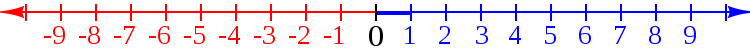
\includegraphics[width=\textwidth]{num.png}
\subsection{Example}
Represent the following equations on the number line.
\[3+5=8\]
\[3-5=-2\]
\[-3+5=2\]
\[-3-5=-8\]	

\section{Multiplication of Negative Numbers}
The multiplication involving negative numbers is summarised below.
\[\begin{array}{c|c|c|}
    \times&1&-1\\
    \hline
    1&1&-1\\
    \hline
    -1&-1&1\\
    \hline
\end{array}\]
\\
Fact: \(-a=(-1)\times a\).
\subsection{Example}
Compute the following.
\[5\times7,(-5)\times7,5\times(-7),(-5)\times(-7)\]
\section{Order of Operations}
By convention, the order of operations is as follows.
\begin{enumerate}
    \item Operations in the inner-most bracket.
    \item Powers.
    \item Multiplications and divisions, from left to right.
    \item Additions and subtractions, from left to right.
\end{enumerate}
\subsection{Example}
Compute the following.
\[2\times(3-4)^3+8\div2^2\]
\[\left(-5-\left(7+(-2)^2\right)\right)\times(-2)\]
\[\left(\left(\frac56-\frac14\right)\div\frac43\right)\times\left(-\frac23\right)^2\]
\end{document}
